\section{Enunciado}

Este trabajo consistirá en analizar los siguientes circuitos con amplificadores operacionales en diferentes configuraciones y además en aplicaciones tanto lineales como no-lineales, todo el análisis se hará con el modelo ideal de los mismos.\\
Se considerará demás lo siguiente:\\
\begin{center}
    $V_C = (V_1 + V_2)/2$\\
$V_D = (V_2 - V_1)$\\
\end{center}

\subsection{Circuito 1: Amplificador Diferencial}
    \subsubsection{Circuito}
        \begin{figure}[ht]
    	\centering
    	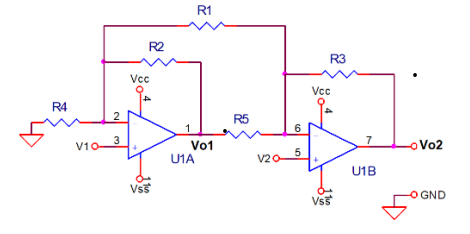
\includegraphics[height=5cm]{Imágenes/AO1.png}
    	\caption{Amplificador Diferencial}
        \end{figure}
    	\begin{center}
            \textbf{Datos:}
        \end{center}
        \begin{itemize}
            \item LM324
            \item $V_{cc}= 10 [V]$
            \item $V_{ss}= -10 [V]$
            \item $R_1 = R_2 = R_3 = R_4 = R_5 = R$
        \end{itemize}
     
     \subsubsection{Análisis}
        \begin{itemize}
            \item $V_{01} = f(V_1, V_2)$
            \item $V_{01} = f(V_D, V_C)$
            \item $V_{02} = f(V_1, V_2)$
            \item $V_{02} = f(V_D, V_C)$
            \item Impedancias vistas desde la fuente de señal
        \end{itemize}

    \subsubsection{Mediciones-Simulaciones}
        \begin{itemize}
            \item Gráfico Entrada/Salida: $V_{01} = f(V_1)$ y $V_{01} = f(V_2)$, $V_{ss}<V_1$, $V_{2}<V_{cc}$ 
            \item Gráfico Entrada/Salida: $V_{01} = f(V_C)$ y $V_{02} = f(V_C)$, $V_{ss}<V_C<V_{cc}$ 
        \end{itemize}

\subsection{Circuito 2: Fuente de Corriente Controlada por Tensión}
    \subsubsection{Circuito}
    	\begin{center}
            \textbf{Datos:}
        \end{center}
        \begin{itemize}
            \item LM324
            \item $V_{cc}= 10 [V]$
            \item $V_{ss}= -10 [V]$
            \item $R_1 = 100 \Omega, R_2 = 10k\Omega, R_3 = 1k\Omega, R_4 = 100k\Omega.$
        \end{itemize}
    	\begin{figure}[ht]
    		\centering
    		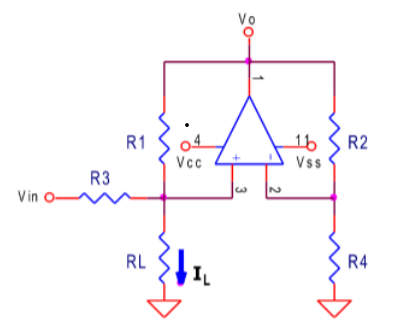
\includegraphics[height=5cm]{Imágenes/AO2.png}
    		\caption{Fuente de Corriente}
    	\end{figure}
     
     \subsubsection{Análisis}
        \begin{itemize}
            \item $I_{RL} = f(R_L, V_{in}), V_o = f(V_{in}, R_L)$
            \item $R_{LMax} = f(V_{in})$
        \end{itemize}
        Completar la siguiente tabla con Mediciones/Simulaciones.\\
        \begin{figure}[ht]
    		\centering
    		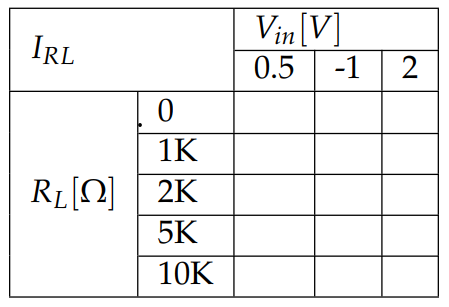
\includegraphics[height=3cm]{Imágenes/Tabla.png}
    	\end{figure}

\subsection{Circuito 3: Rectificador de Precisión}
    \subsubsection{Circuito}
    	\begin{center}
            \textbf{Datos:}
        \end{center}
        \begin{itemize}
            \item LM324
            \item $V_{cc}= 10 [V]$
            \item $V_{ss}= -10 [V]$
            \item $D_1 = D_2 = 1N4148$
            \item $R_1 = R_3 = R_4 = 10k\Omega-1\%$ y $ R_2 = 5K\Omega-1\% $
        \end{itemize}
    	\begin{figure}[ht]
    		\centering
    		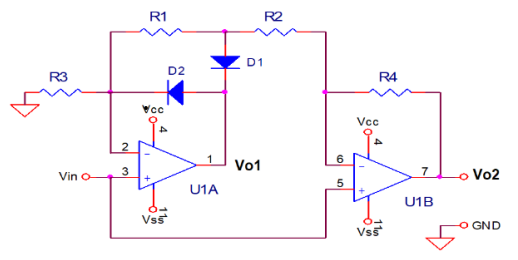
\includegraphics[height=4cm]{Imágenes/AO3.png}
    		\caption{Rectificador de Precisión}
    	\end{figure}
     
     \subsubsection{Análisis}
        \begin{itemize}
            \item $V_{01} = f(V_{in})$, $V_{02} = f(V_{in})$, con $0V<V_{in}$ (Ignorar Rd del Diodo).
            \item $V_{01} = f(V_{in})$, $V_{02} = f(V_{in})$, con $V_{in}>0V$ (Ignorar Rd del Diodo).
        \end{itemize}

    \subsubsection{Mediciones-Simulaciones}
        \begin{itemize}
            \item Gráfico Entrada/Salida: $V_{01} = f(V_{in})$ y $V_{02} = f(V_{in})$, $V_{ss}<V_1<V_{cc}$ 
        \end{itemize}
        
\subsection{Circuito 4: Comparador con Histéresis}
    \subsubsection{Circuito}
    	\begin{center}
            \textbf{Datos:}
        \end{center}
        \begin{itemize}
            \item LM324
            \item $V_{+} = 10 [V]$
            \item $V_{-} = 0 [V]$
            \item $R_1 = R_2 = R_4 = 10k\Omega, R_3 = 2K\Omega$
            \item $V_{ref} = 2 [V]$
        \end{itemize}
    	\begin{figure}[ht]
    		\centering
    		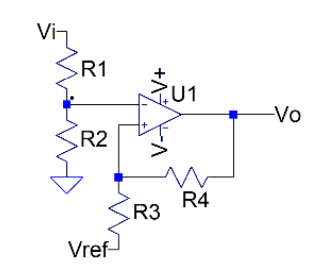
\includegraphics[height=5cm]{Imágenes/AO4.png}
    		\caption{Comparador con Histéresis}
    	\end{figure}
     
     \subsubsection{Análisis}
        \begin{itemize}
            \item Umbral de conmutación cuando $V_o = V_+$.
            \item Impedancia vista por las fuentes de señal
        \end{itemize}

    \subsubsection{Mediciones-Simulaciones}
        \begin{itemize}
            \item Gráfico Entrada/Salida: $V_{o} = f(V_{in}), V_-<V_c<V_+$ 
        \end{itemize}
        
\subsection{Ejercicio Adicional I}
Diseñar un regulador de carga de batería, que corte cuando se alcanzan los 12.8V y reinicie la
carga cuando baja a 10.5V.\\
\begin{center}
    \textbf{Materiales:}\\
\end{center}
    \begin{itemize}
        \item AO ideal con Saturación.
        \item Resistencias.
        \item 1 Relé 12V, Normal Abierto, 20mA de corriente de bobina.
        \item 1 Transistor NPN BC548 o PNP BC558.
        \item 1 Diodo 1N4148.
        \item 1 Referencia de Tensión: TL431.
        \item Batería 12V (Rango 8V a 13V) - $R_{in} = 0.5 \Omega$.
        \item Celda Fotovoltaica: 15V Tensión sin carga, 1A de corriente de carga.
    \end{itemize}
    
\subsection{Ejercicio Adicional II}
Diseñar un oscilador de relajación que oscile a 1kHz.\\
\begin{center}
    \textbf{Materiales:}\\
\end{center}
    \begin{itemize}
        \item AO ideal con Saturación.
        \item Resistencias.
        \item Capacitor de 1uF.
    \end{itemize}
\newpage

\section{Introducción}
Los \textbf{amplificadores operacionales} (conocidos también como \textbf{op-amps}) son dispositivos electrónicos fundamentales en el diseño de circuitos analógicos. Originalmente desarrollados para realizar operaciones matemáticas en computadoras analógicas, hoy en día se utilizan en una amplia gama de aplicaciones, desde amplificación de señales hasta filtros, osciladores y más.\\

\textbf{Características Principales:}
\begin{itemize}
    \item Ganancia de tensión casi infinita: Teóricamente, un op-amp ideal amplifica infinitamente la diferencia de voltaje entre sus entradas.
    \item Impedancia de entrada casi infinita: Permite que fluya una muy pequeña corriente hacia las entradas, lo que evita la carga del circuito previo y simplifica el acoplamiento entre varios de los mismos.
    \item Impedancia de salida casi nula: La salida podría entregar bastante intensidad de corriente con una mínima caída de potencial en su salida.
    \item Rechazo al modo común: Tiene la capacidad de amplificar las tensiones diferenciales, no así las tensiones comúnes a sus terminales, de aquí sale el concepto de la relación de rechazo al modo común.
\end{itemize}

\textbf{Apliciones comúnes:}
\begin{itemize}
    \item Comparadores: Pueden indicar mediante un análisis de la salida, si la tensión en su entrada es mayor a cierto umbral.
    \item Filtros Activos: Mediante un filtro pasivo y un amplificador operacional, es posible mejorar las características del filtro en cuestión.
    \item Amplificadores de señal: Tienen la capacidad de proveer a lazo cerrado una ganacia muy constante y alta, útil en aplicaciones en baja señal.
    \item Adaptaciones de señal: Mediante operaciones matemáticas aplicadas analógicamente a la señal, es posible adaptar una señal de entrada a los requerimientos que se poseen.
    \item Osciladores: Pueden ser utilizados para generar señales periódica, como onda sinusoidales, cuadradas, triangulares, de los mismos surge el famoso integrado "555".
    \item Etc.
\end{itemize}

Los amplificadores operacionales son componentes versátiles y esenciales en el diseño de circuitos analógicos, gracias a su capacidad para ser configurados de diversas maneras y su utilidad en una multitud de aplicaciones electrónicas.


\newpage
\section{Desarrollo}
    \subsection{Circuito 1:}
    \begin{figure}[ht]
    	\centering
    	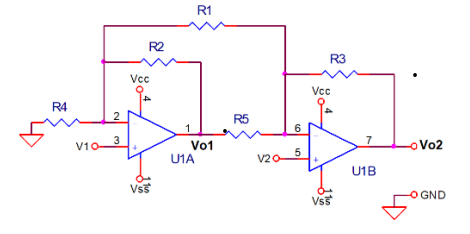
\includegraphics[height=5cm]{Imágenes/AO1.png}
    	\caption{Amplificador Diferencial}
    \end{figure}
    
        \subsubsection{Análisis}
        En este circuíto se propondrá que el mismo está en la zona lineal, ahora con este suposición aplicamos el método de superposición para obtener la salida: \\
        
        $V_{01}|_{V_2=0} = (1+\frac{R_2}{R_1//R_4}).V_1 = (1+\frac{R}{R/2}).V_1 = 3V_1 $\\
        
        $V_{01}|_{V_1=0} = -(\frac{R_2}{R_1}).V_2 = -V_2 $\\
        
        $V_{02}|_{V_1=0, V_{01}=0} = (1+\frac{R_3}{R_1//R_5}).V_2 = (1+\frac{R}{R/2}).V_2 $\\
        
        $V_{02}|_{V_2=0, V_{01}=0} = -(\frac{R_3}{R_1}).V_1 = -V_1 $\\
        
        $V_{02}|_{V_1=0, V_2=0} = -(\frac{R_3}{R_5}).V_{01} = -V_{01} $\\
        
       \textbf{ Entonces:}\\
        
        $V_{01} =  3V_1 - V_2$\\
        
        $V_{02} =  3V_2 - V_1 -V_{01} = 3V_2 - V_1 -3V_1 + V_2 = 4(V_2-V_1) $\\

        \begin{center}
            \boxed{V_{01} =  3V_1 - V_2}\\
            \boxed{V_{02} = 4(V_2-V_1)}\\
        \end{center}

        Ahora si reemplazamos $V_D = (V_2 - V_1)$, se obtendrá:\\
        
        \begin{center}
            \boxed{V_{02} = 4V_D}\\
        \end{center}
        
        Pero si se reemplaza con una tensión común $V_1 = V_2$, con $V_C = (V_1 + V_2)/2$:\\
        
        \begin{center}
            \boxed{V_{02} = 0}\\  
        \end{center}

        Por lo que la relación de rechazo al modo común \textbf{RRMC} daría en este caso:\\
        
        \begin{center}
            \boxed{RRMC = \frac{V_D}{V_C} = \infty}\\
        \end{center}

        Para el análisis de las \textbf{impedancias} vistas por cada entrada, se supone que el amplificador operacional es \textbf{ideal}, por lo cual:\\

        \begin{center}
            \boxed{Z_{i1} = \frac{V_1}{I_{i1}} = \infty}\\
            \boxed{Z_{i2} = \frac{V_2}{I_{i2}} = \infty}\\
        \end{center}

        La impedancia de salida será:\\

        \begin{center}
            \boxed{Z_{o} = \frac{V_0}{I_{o}} = 0}\\
        \end{center}
        
        \subsubsection{Simulación}
        Se realizaron difetentes simulaciones en \textbf{LTSpice} observando el comportamiento de cada salida del AO:\\

        \begin{figure}[ht]
        	\centering
        	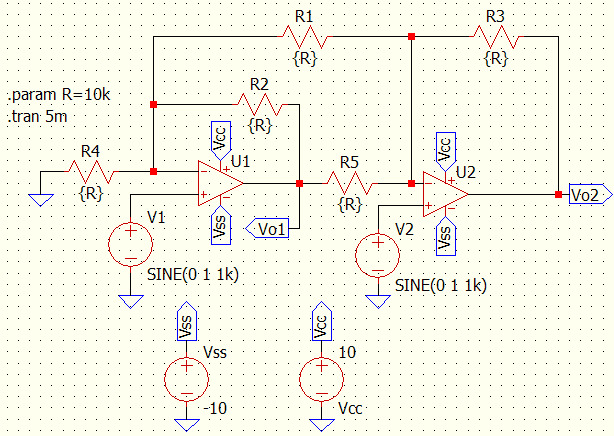
\includegraphics[height=10cm]{Imágenes/EJ1.1.jpeg}
        	\caption{Circuíto Simulado en LTSpice}
        \end{figure}
    
        \begin{figure}[ht]
        	\centering
        	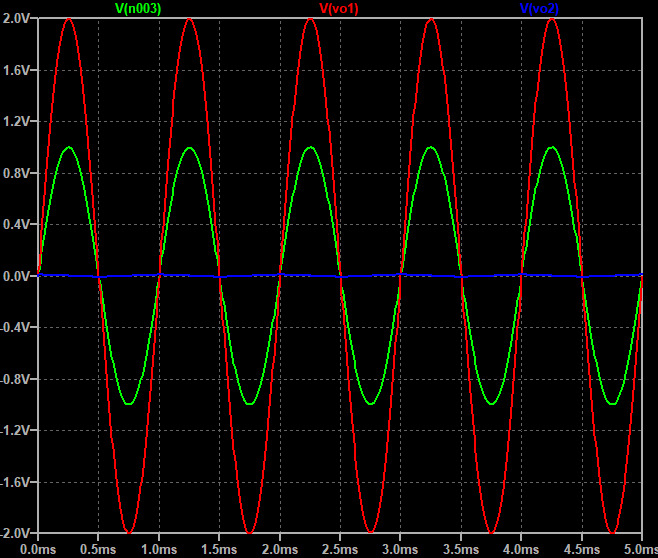
\includegraphics[height=6cm]{Imágenes/EJ1.jpeg}
        	\caption{Salida del AO}
        \end{figure}

        \begin{figure}[H]
        	\centering
        	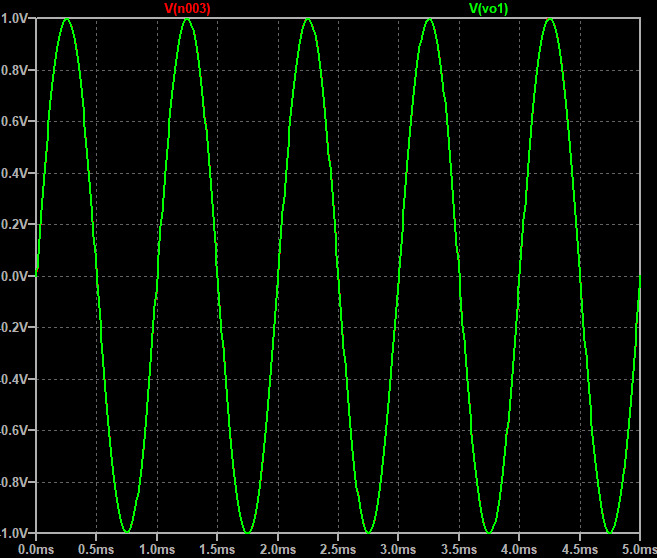
\includegraphics[height=6cm]{Imágenes/EJ1.2.jpeg}
        	\caption{$V_{in1}$ y $V_{o1}$}
        \end{figure}

        \begin{figure}[H]
        	\centering
        	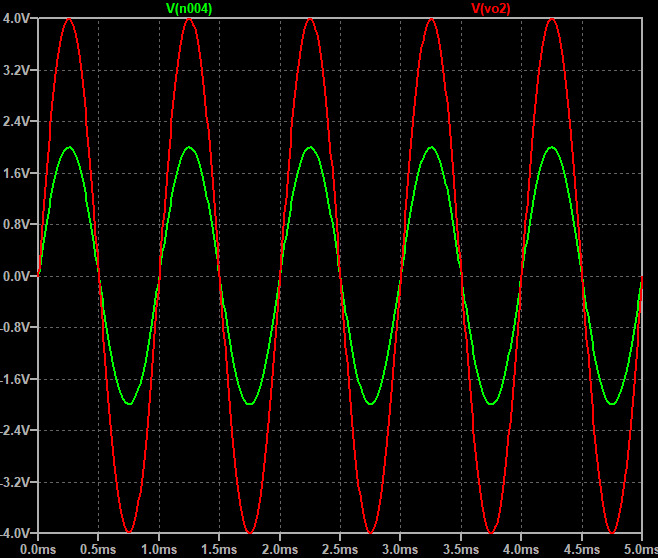
\includegraphics[height=6cm]{Imágenes/EJ1.3.jpeg}
        	\caption{$V_{in2}$ y $V_{o2}$}
        \end{figure}


    \newpage
    \subsection{Circuito 2:}
    \begin{figure}[ht]
    	\centering
    	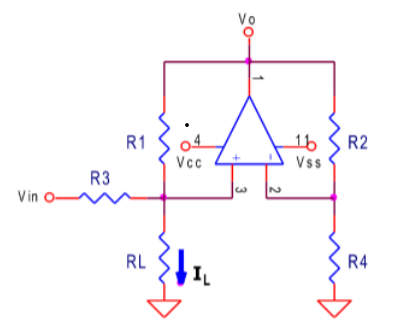
\includegraphics[height=5cm]{Imágenes/AO2.png}
    	\caption{Fuente de Corriente controlada por Tensión}
    \end{figure}
        \subsubsection{Análisis}
        Para analizar este circuito, simplemente hacemos las ecuaciones de nodo, si tomamos la ganancia del operacional como ideal(infinita) y además que el mismo se encuentra en la zona lineal, podemos tomar que $V+ = V-$:\\
        Entonces:\\
        
        $0 = \frac{V_{-}}{R_{4}} + \frac{- V_{o} + V_{-}}{R_{2}}$\\
        
        $0 = \frac{V_{+}}{R_{L}} + \frac{- V_{in} + V_{+}}{R_{3}} + \frac{- V_{o} + V_{+}}{R_{1}}$\\

        $I_L = \frac{V_{+}}{R_L}$\\

        Si de estas expresiones, se igualan, podremos hayar la relación entre la corriente en la carga $I_L$ y la tensión de entrada $V_{in}$:\\
        
        \begin{center}
            \boxed{I_{L} = \frac{R_{1} R_{4} V_{in}}{R_{1} R_{3} R_{4} + R_{1} R_{4} R_{L} - R_{2} R_{3} R_{L}}}\\
        \end{center}

        Ahora para determinar los límites de este circuito, debemos conocer la tensión de salida $V_o$

        \begin{center}
            \boxed{V_{o} = \frac{R_{1} R_{L} V_{in} \left(R_{2} + R_{4}\right)}{R_{1} R_{3} R_{4} + R_{1} R_{4} R_{L} - R_{2} R_{3} R_{L}}}\\
        \end{center}

        Con este dato, si tomamos que $V_{omax} = Vcc*0.9$ y se reemplaza por cada valor de resistencia dado, podemos hayar cuanto será $R_{Lmax}$:\\

        \begin{center}
            \boxed{R_{Lmax} = \frac{818.2*V_{cc}}{V_{in}}}\\
        \end{center}

        Este será el valor máximo de resistencia de carga de manera que la tensión de salida no supere la de alimentación, evitando así que el operacional no entre en saturación. Bajo esta condición, la corriente en la carga será:\\

        \begin{center}
            \boxed{I_{L} = 0.001*V_{in}}\\
        \end{center}
        
        \subsubsection{Simulación}

        \begin{figure}[H]
        	\centering
        	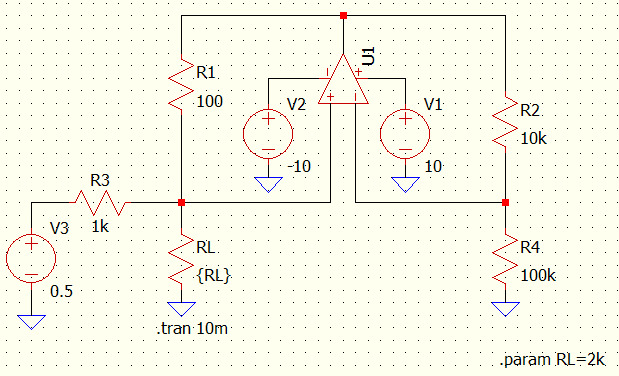
\includegraphics[height=8cm]{Imágenes/Ej2.jpeg}
        	\caption{Circuíto a simular}
        \end{figure}

        \begin{figure}[H]
        	\centering
        	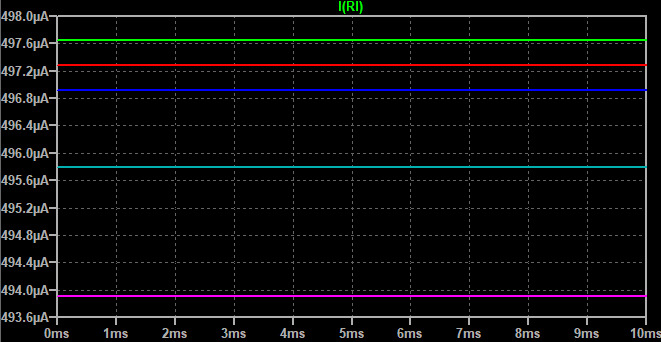
\includegraphics[height=6cm]{Imágenes/EJ2_CASO1.jpeg}
        	\caption{Caso 1, $V_{in} = 0.5 [V]$}
        \end{figure}

        \begin{figure}[H]
        	\centering
        	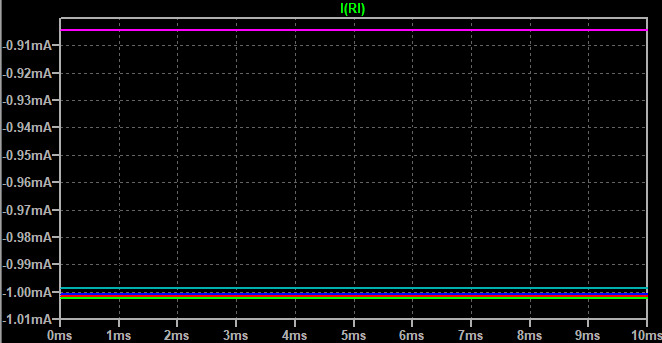
\includegraphics[height=6cm]{Imágenes/EJ2_CASO2.jpeg}
        	\caption{Caso 2, $V_{in} = -1 [V]$}
        \end{figure}

        \begin{figure}[H]
        	\centering
        	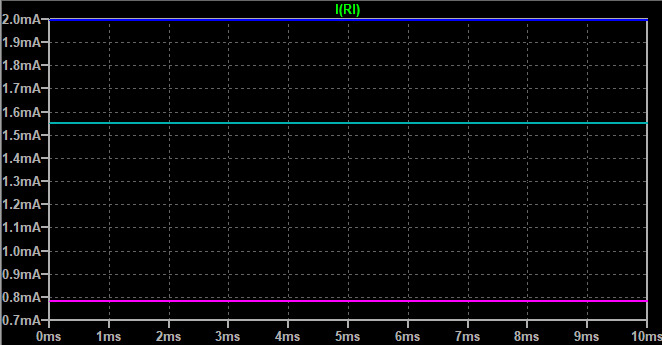
\includegraphics[height=6cm]{Imágenes/EJ2_CASO3.jpeg}
        	\caption{Caso 3, $V_{in} = 2 [V]$}
        \end{figure}
        
    \subsection{Circuito 3:}
        \begin{figure}[ht]
        	\centering
        	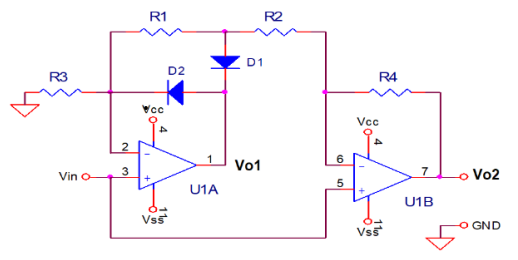
\includegraphics[height=5cm]{Imágenes/AO3.png}
        	\caption{Rectificador de Precisión}
        \end{figure}
        
        \subsubsection{Análisis}
        Para realizar el análisis, debemos tomarlo en dos partes, para una tensión de entrada positiva, es decir, para \textbf{$V_{in}>0$} entonces:\\
        
        \begin{figure}[ht]
        	\centering
        	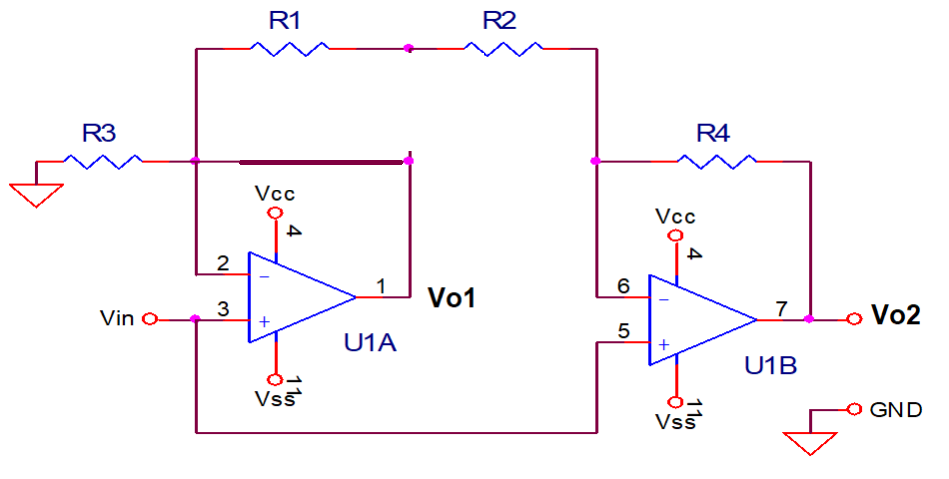
\includegraphics[height=4cm]{Imágenes/C3_pos.png}
        	\caption{En tensiones Positivas}
        \end{figure}
        
        De aquí saldrán estas dos ecuaciones de nodos:\\
        
        $0 = \frac{V1_{+} - V2_{+}}{R_{1} + R_{2}} + \frac{V1_{+}}{R_{3}}$\\
        
        $0 = \frac{-V1_{+} + V2_{+}}{R_{1} + R_{2}} + \frac{-V_{02} + V2_{+}}{R_{4}}$\\

        Si aplicamos superposición:\\

        \begin{center}
            \boxed{V_{02} = 1.66666*V_{in} - 0.666666*V_{in} = 1.0*V_{in}}\\
        \end{center}
        
        Ahora si analizamos nuevamente pero para una tensión de entrada negativa, es decir, para \textbf{$V_{in}<0$} entonces:\\
        \begin{figure}[ht]
        	\centering
        	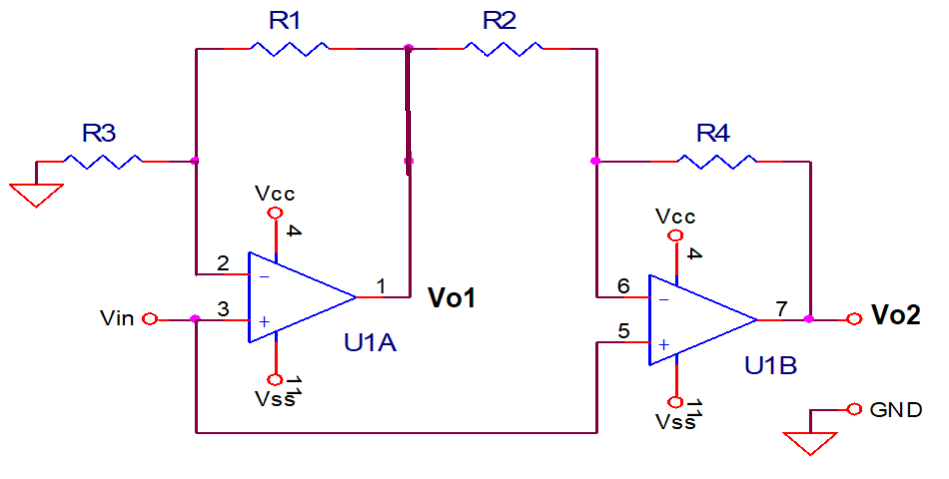
\includegraphics[height=4cm]{Imágenes/C3_neg.png}
        	\caption{En tensiones Negativas}
        \end{figure}

        De aquí saldrán estas dos ecuaciones de nodos:\\
        
        $0 = \frac{V1_{+}}{R_{3}} + \frac{-V_{01} + V1_{+}}{R_{1}}$\\
        
        $0 = \frac{-V_{02} + V2_{+}}{R_{4}} + \frac{-V_{01} + V2_{+}}{R_{2}}$\\

        Si aplicamos superposición:\\

        \begin{center}
            \boxed{V_{02} = 3*V_{in} - 4*V_{in} = -1.0*V_{in}}\\
        \end{center}
        
        
        \subsubsection{Simulación}
        
        \begin{figure}[ht]
        	\centering
        	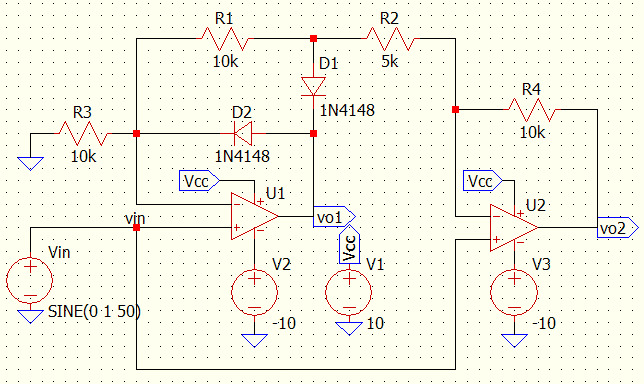
\includegraphics[height=8cm]{Imágenes/EJ3.jpeg}
        	\caption{Circuíto a Simular}
        \end{figure}

        \begin{figure}[ht]
        	\centering
        	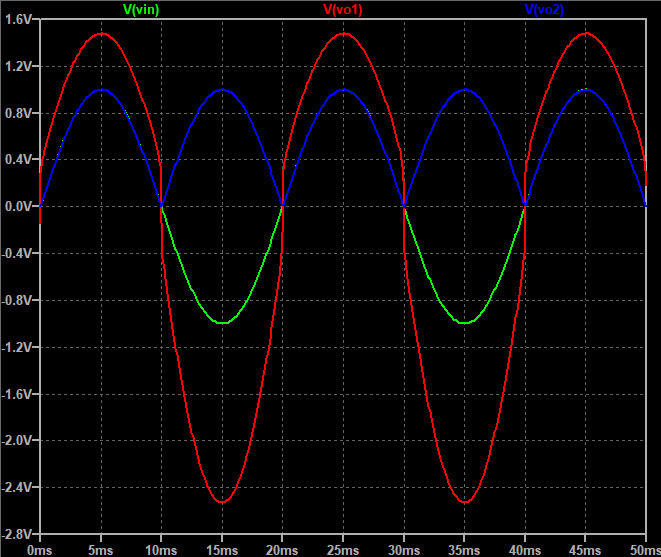
\includegraphics[height=8cm]{Imágenes/EJ3.1.jpeg}
        	\caption{Salida}
        \end{figure}
        
        
    \subsection{Circuito 4:}
        \begin{figure}[ht]
        	\centering
        	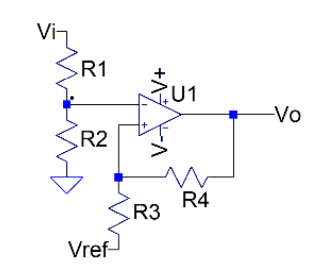
\includegraphics[height=5cm]{Imágenes/AO4.png}
        	\caption{Comparador con Histéresis}
        \end{figure}
        \subsubsection{Análisis}
        Este es un circuíto comparador con histéresis inversor "Schmitt Trigger Inversor", puesto con una fuente de alimentación asimétrica; Se comienza el análisis partiendo de que:\\

        $V_{-} = V_{in}*\frac{R_{2}}{R_{2} + R_{1}}$\\
        
        $V_{+} = V_{o}*\frac{R_{3}}{R_{3} + R_{4}} + V_{ref}*\frac{R_{4}}{R_{3} + R_{4}}$\\

        Ahora si $V_{d} = V_{+} - V_{-}$, y tomamos que  $V_{d} > 0$, entonces:\\

        $V_{o} = V_{cc}$\\
        
        $V_{+} > V_{-},   V_{o}*0.166 + V_{ref}*0.833 > V_{in}*0.5$\\

        \begin{center}
            \boxed{V_{in} > 6.667 [V], \xrightarrow{} V_{o} = 10 [V]}\\
        \end{center}


        Pero con $V_{d} < 0$, entonces:\\

        $V_{o} = V_{ss} = 0[V]$\\
        
        $V_{+} < V_{-},  V_{ref}*0.833 < V_{in}*0.5$\\

        \begin{center}
            \boxed{V_{in} < 3.33 [V], \xrightarrow{} V_{o} = 0 [V]}\\
        \end{center}

        Ahora si $V_{d} = 0$, entonces:\\

        $V_{o} = 0$\\
        
        $V_{+} = V_{-}, V_{ref}*0.833 = V_{in}*0.5$\\

        \begin{center}
            \boxed{V_{in} = 3.33 [V], \xrightarrow{} V_{o} = 0 [V]}\\
        \end{center}

        \newpage
        \subsubsection{Simulación}

        \begin{figure}[ht]
        	\centering
        	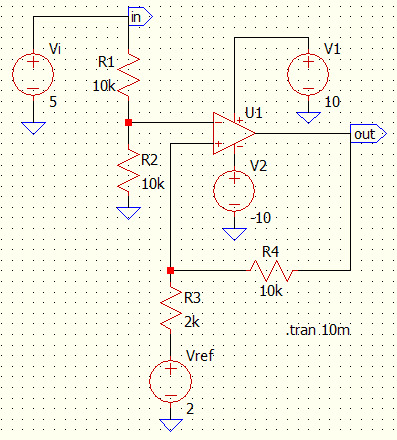
\includegraphics[height=6.5cm]{Imágenes/EJ4.jpeg}
        	\caption{circuíto en LTSpice}
        \end{figure}

        \begin{figure}[ht]
        	\centering
        	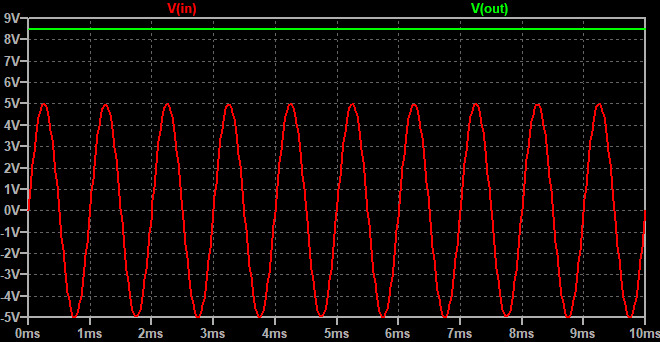
\includegraphics[height=8cm]{Imágenes/EJ4.1.jpeg}
        	\caption{Salida}
        \end{figure}
 
	\newpage

	